\documentclass{report}

\usepackage[utf8]{inputenc}
\usepackage[letterpaper,top=2cm,bottom=2cm,left=3cm,right=3cm,marginparwidth=1.75cm]{geometry}
\usepackage{graphicx}

\title{PDF report}
\author{Maksim Al Dandan}
\date{\today}

\begin{document}
\maketitle
\newpage

\section*{Design patterns}
\subsection*{Creational patterns}

I used Factory pattern to create different types of users. I have two types of accounts: standard and premium. Hence, I created UserFactory class that creates different types of users based on the type of account.

\subsection*{Structural patterns}

I used Proxy pattern as an intermidiary between the user input and buiseness logic. The Proxy class is responsible for validating the user input and then passing it to the buiseness logic.

\subsection*{Behavioral patterns}

I used observer pattern to create a notification system. Users can subscribe to the notification system and receive notifications book price changes. Class Publisher is responsible for notifying all the subscribers about the price change.

\section*{UML diagram}

To see the UML diagram, please refer to the next page.

\newpage
\begin{figure}[h]
    \centering
    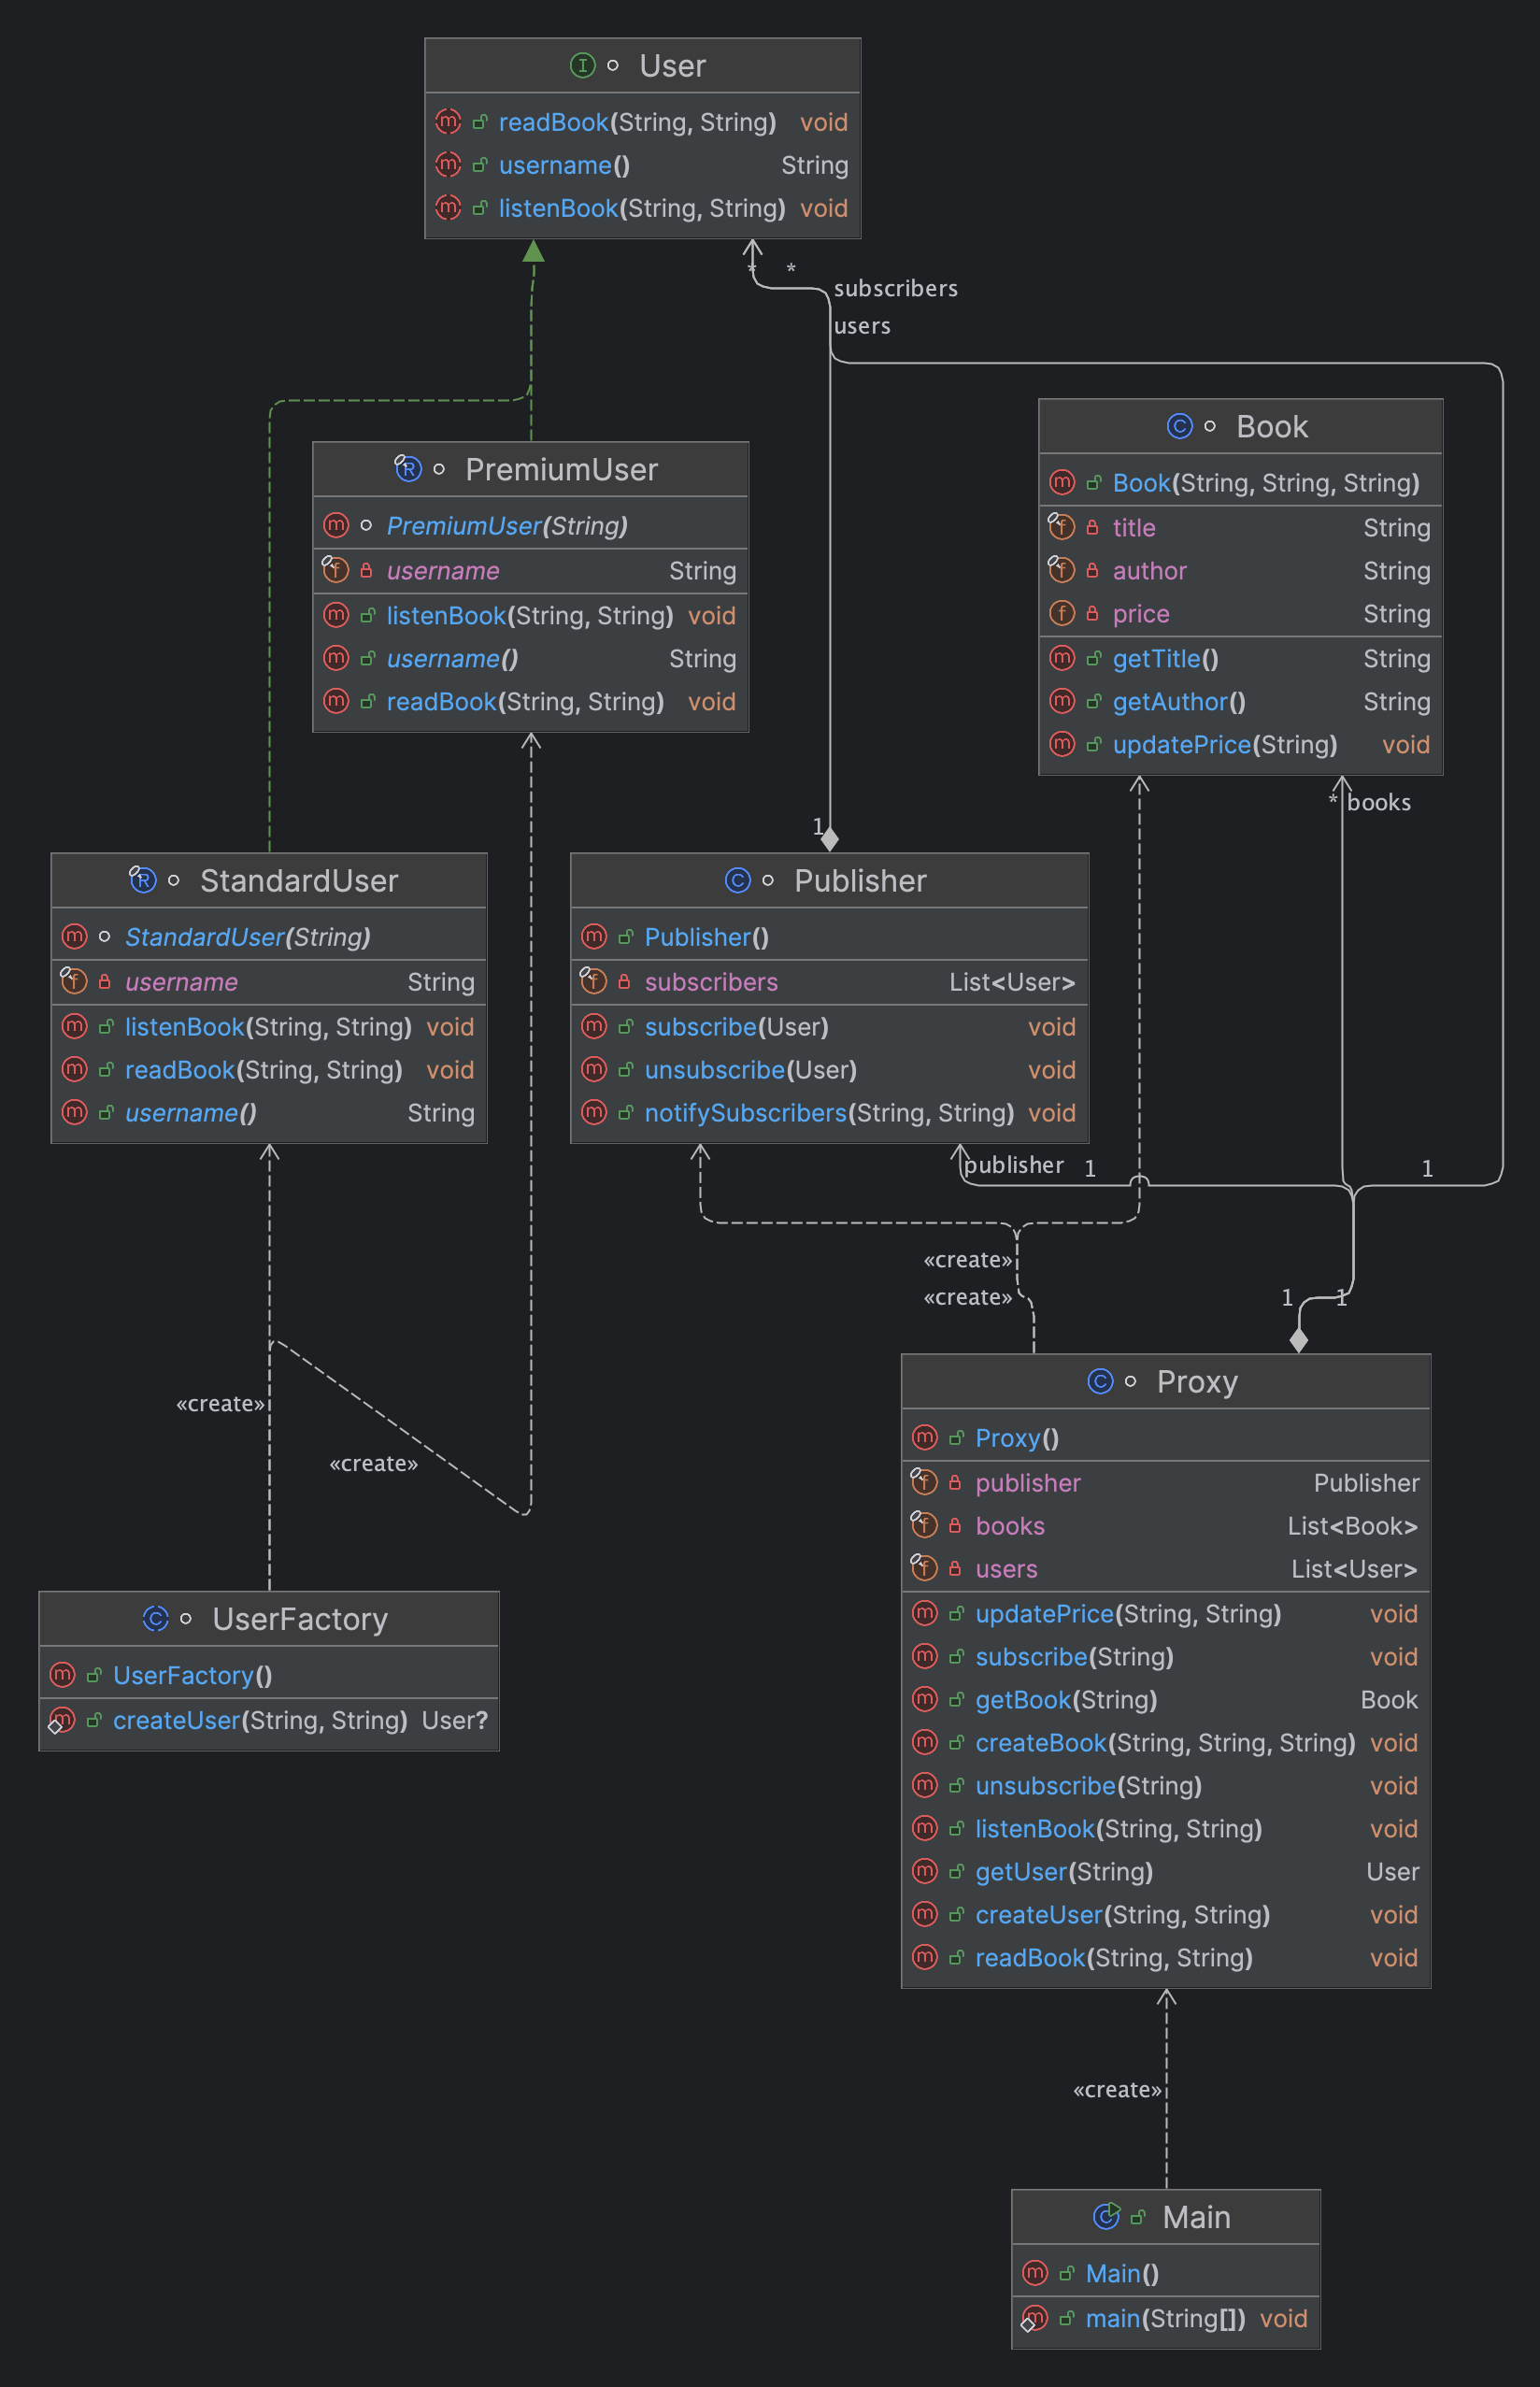
\includegraphics[width=\textwidth]{UML.png}
    \caption{UML diagram}
\end{figure}

\end{document}
